%This is the presentation template Christine P'ng made (and uses)
%It uses a different theme and different fonts

\documentclass{beamer}
%\documentclass[handout]{beamer}

%\usetheme{Boadilla}

\usepackage{libertine}
\usepackage[T1]{fontenc}
\usepackage[utf8x]{inputenc}
\usepackage[french]{babel}
\usepackage{subfig}
\usepackage{xcolor}
\usepackage{colortbl}
\usepackage{listings}
\usepackage{tikz}
\usepackage{marvosym}
%\usepackage{tikzsymbols}
 \usepackage[marvosym]{tikzsymbols}
\usetikzlibrary{arrows.meta}
\usepackage{environ}
\usepackage{multirow}
\usepackage{multicol}
\usepackage{rotating}
\usepackage[ampersand]{easylist}
\usepackage{wasysym}
\usepackage{booktabs}
\usepackage{centernot}
\usetikzlibrary{shapes,arrows,decorations.pathmorphing,decorations.pathreplacing,backgrounds,positioning,fit,petri}
\usepackage{ulem}
\usepackage{cancel}
\usepackage{tikz}
\usetikzlibrary{arrows}
\usepackage{appendixnumberbeamer}

\definecolor{gcblue}{RGB}{66,126,214} % sampled with Gimp
\definecolor{customRed}{RGB}{240,80,80}
\definecolor{faintred}{RGB}{255,175,175}
\definecolor{faintblue}{RGB}{110,220,255}
\definecolor{faintgray}{RGB}{225,225,225}
\definecolor{titlefontblue}{RGB}{45,45,80}
\definecolor{titlefontcolour}{RGB}{75,75,75}

\usecolortheme[named=titlefontcolour]{structure}
\setbeamersize{text margin left=10mm}
\setbeamertemplate{frametitle}{\vspace{1.5cm}\insertframetitle}
\usefonttheme{serif} %serif

%Setting a different font family for the title and frame titles
%Short titles and headers are required because the font size is set to very large (feel free to change this based on presentation requirements)
% ##### \setbeamerfont{title}{family=\fontfamily{cmr}}
\setbeamerfont{title}{family=\fontfamily{cmss}}
\setbeamerfont{title}{family=\sffamily} %sffamily
\setbeamerfont{title}{size=\fontsize{33}{33}\bfseries}%make this smaller if your title is too long (do the same for the frametitles, etc)
\setbeamerfont{frametitle}{family=\sffamily}
\setbeamerfont{frametitle}{size=\Huge\bfseries}
\setbeamerfont{author}{size=\normalsize\scshape}
\setbeamerfont{institute}{size=\small\scshape}
\setbeamerfont{date}{size=\small\scshape}
\setbeamerfont{subtitle}{size=\small}
\setbeamerfont{normal text}{size=\Huge}

\setbeamertemplate{navigation symbols}{}
\setbeamertemplate{footline}[frame number]{}
\setbeamertemplate{itemize items}[ball]
%\setbeamercolor{itemize items}{fg=blue}
%\setbeamertemplate{itemize item}{\color{yellow}$\blacksquare$}

%\setbeamercolor{itemize item}{fg=red}
%\setbeamercolor{itemize item}{bg=red}

%Adding page numbers at the bottom of each frame
%\setbeamertemplate{footline}
%{%
%  \leavevmode%
%  \hbox{%
%  \begin{beamercolorbox}[wd=1\paperwidth,ht=2.25ex,dp=1ex,right]{date in head/foot}%
%   % \usebeamerfont{date in head/foot}\insertshortdate{}\hspace*{2em}
%    \insertframenumber{} / \inserttotalframenumber\hspace*{2ex} 
%  \end{beamercolorbox}}%
%  \vskip0pt%
%}

%Header Info
% information not capitalized because fonts are set to small caps (looks cleaner this way)
%\title[SRSWOR CLT]{
%	\mbox{} \vskip 2.0cm
%	%{\color{white}Statistics + Algebraic Geometry $=$ $?$}
%	\vskip 0.1cm
%	\small
%	%{\color{white}Identifiability}
%	}


%\author{\vskip -1.5cm\LARGE%\color{titlefontcolour}
%Kenneth Chu}

%\institute[oicr]{\scriptsize
%	\color{titlefontcolour}
%	\inst{}
%	Special Surveys, Transportation, Technology and Quality Assurance, BSMD
%	\vskip 0.0cm
%	Enqu\^{e}tes sp\'{e}ciales, transport, technologie et assurance de la qualit\'{e}, DMEE
%	}

%\date{\color{titlefontcolour}October 21, 2015} 

%%%%%%%%%%%%%%%%%%%%%%%%%%%%%%%%%%%%%%%%%%%%%%%%%%
\begin{document}

\addtocounter{framenumber}{-1}
{
% Titlepage
\usebackgroundtemplate{
\includegraphics[width=\paperwidth,height=\paperheight]{StatCan-presentation-titlePage-background.jpg}}
\begin{frame}[plain]
%\titlepage

\begin{center}

\vskip 3.5cm
\resizebox{0.75\linewidth}{!}{\color{titlefontblue}\bf\itshape Le Bitcoin}
\vskip 0.2cm
\resizebox{0.75\linewidth}{!}{\color{titlefontblue}\bf\itshape et la Cha\^ine de blocs}
%\textbf{\huge\color{titlefontblue} et la Cha\^ine de blocs}

\vskip 0.5cm
\textbf{\large\color{titlefontcolour}Kenneth Chu}

\vskip 0.2cm
\textbf{\scriptsize\color{titlefontcolour}Centre de ressources en analyse de donn\'{e}es, DCIMSI
\vskip -0.1cm
Data Analysis and Resource Centre, ICCSMD}

\vskip 0.2cm
\textbf{\color{titlefontcolour}25 avril 2017} 

\end{center}

\end{frame}
}

% Outline
%\begin{frame}{Outline}
%\tableofcontents
%\end{frame}

%%%%%%%%%%%%%%%%%%%%%%%%%%%%%%%%%%%%%%%%%%%%%%%%%%
\newcommand{\graphicsDir}{graphics}
\newcommand*\rot{\rotatebox{90}}
\renewcommand{\Re}{\mathbb{R}}
\newcommand{\N}{\mathbb{N}}
\renewcommand{\d}{\textnormal{d}}
\newcommand{\Var}{\textnormal{Var}}

\definecolor{bgOrange}{RGB}{255,229,204}
\definecolor{lightOrange}{RGB}{220,153,136}
\definecolor{lightBlue}{RGB}{0,200,200}
\definecolor{darkBlue}{RGB}{40,80,204}
\definecolor{lessDeepGreen}{RGB}{0,201,100}
\definecolor{deepGreen}{RGB}{0,115,57}
\definecolor{darkYellow}{RGB}{200,200,0}
\definecolor{lightTurquoise}{RGB}{153,255,255}
\definecolor{lightYellow}{RGB}{255,255,204}
\definecolor{lightGreen}{RGB}{204,255,204}
\definecolor{darkGreen}{RGB}{128,255,0}
\definecolor{veryDarkGreen}{RGB}{100,225,100}
\definecolor{lightGray}{RGB}{224,224,224}
\definecolor{mediumLightGray}{RGB}{176,176,176}
\definecolor{mediumGray}{RGB}{128,128,128}

\setlength{\arrayrulewidth}{0.55pt}
\arrayrulecolor{mediumGray}

%%%%% ~~~~~~~~~~~~~~~~~~~~ %%%%%
\usebackgroundtemplate{
\includegraphics[width=\paperwidth,height=0.0825\paperwidth]{StatCan-presentation-body-topBanner.jpg}}

%\setlength{\parskip}{0.3cm}


%%%%%%%%%%

\begin{frame}{\vskip -0.2cm\Large Premier achat document\'e d'un objet physique gr\^ace \`a des bitcoins}

\begin{multicols}{2}

	\begin{flushleft}
	\mbox{}\vskip -0.4cm
	%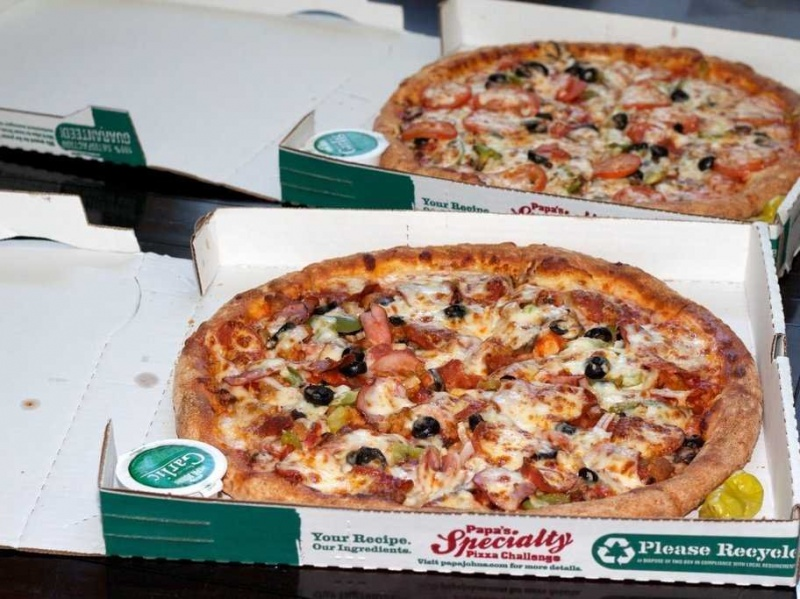
\includegraphics[width=12cm]{graphics/800px-Laszlospizza.jpg}
	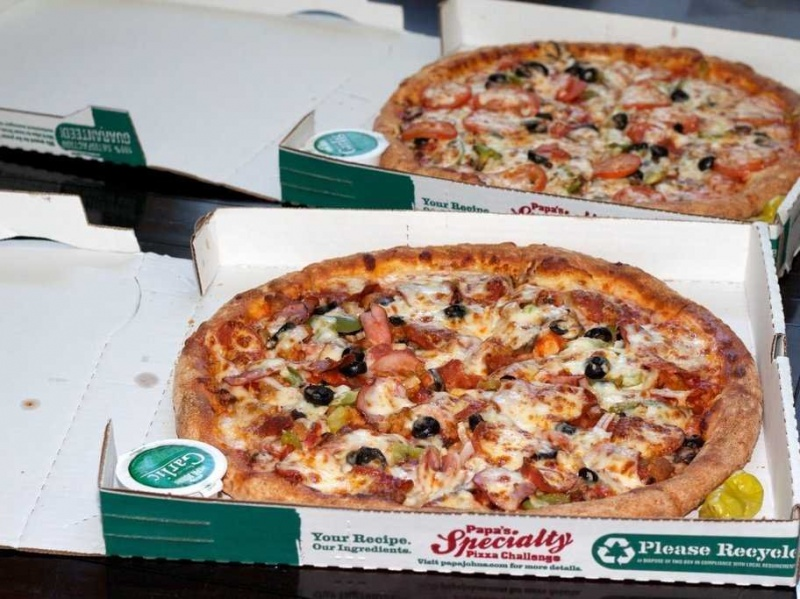
\includegraphics[height=5.5cm]{graphics/800px-Laszlospizza.jpg}
	\vskip -0.1cm
	{\tiny\texttt{https://en.bitcoin.it/wiki/Laszlo\_Hanyecz}}
	\vskip -0.2cm
	{\tiny\texttt{https://bitcointalk.org/index.php?topic=137.msg1195\#msg1195}}
	
	\end{flushleft}

\columnbreak

	\begin{flushright}

		\begin{minipage}{2.7cm}{\bf
		\begin{center}
		
		\mbox{}\vskip 0.2cm
		{\huge\color{red}2 pizzas}
		\vskip 0.5cm
		{\Large 10,000 BTC}
		\vskip 0.5cm
		{\Large 22 mai 2010}
		\vskip -0.175cm
		{\tiny(Journ\'ee de Pizza Bitcoin)}		
		\vskip 0.5cm
		Laszlo Hanyecz
		\vskip -0.1cm
		{\tiny\begin{itemize}
		\item
			un des premiers mineurs de bitcoin
		\item
			d\'eveloppeur informatique am\'ericain
		\end{itemize}}
				
		\end{center}
    		}\end{minipage}
		
	
	\end{flushright}

\end{multicols}

\normalsize
\end{frame}

%%%%%%%%%%


%%%%%%%%%%

\begin{frame}{\vskip -0.1cm\Large Depuis, une petite diff\'erence}

\begin{columns}
\column{\dimexpr\paperwidth-1pt}

\begin{center}
\vskip -0.2cm
%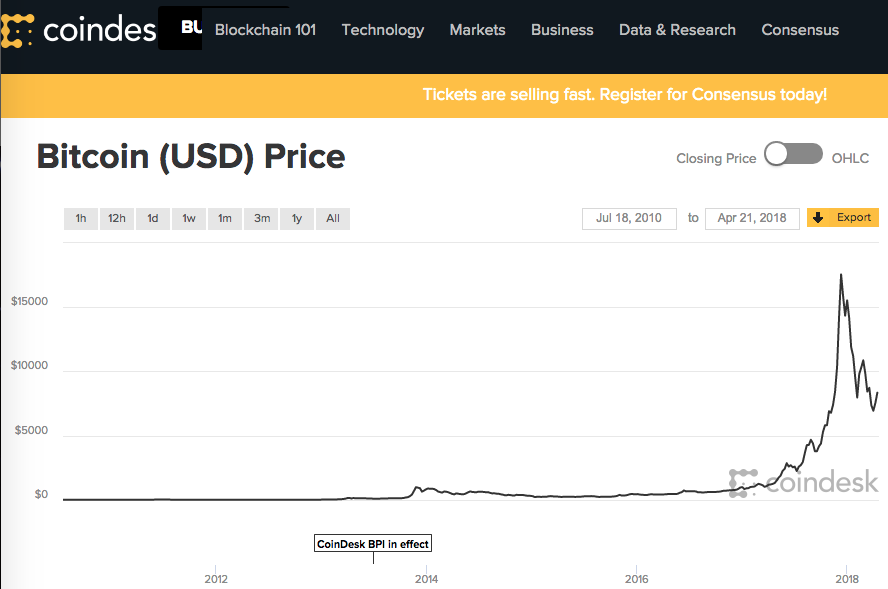
\includegraphics[height=6cm]{graphics/bitcoin-price-chart-coindesk.png}
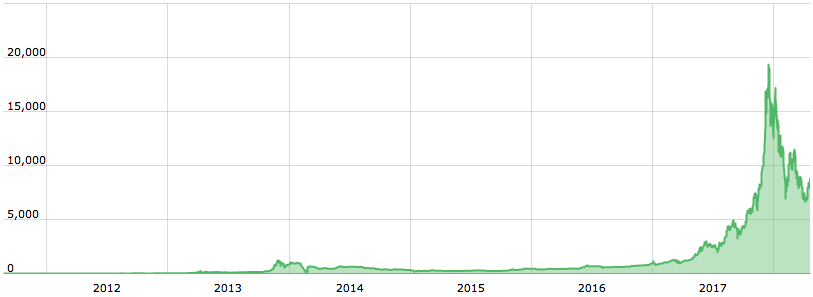
\includegraphics[width=12.25cm]{graphics/bitcoin-price-chart-fr.png}
\vskip -0.1cm
{\tiny\texttt{https://bitcoin.fr/le-cours-du-bitcoin/}}%\texttt{https://www.coindesk.com/price/}

%\vskip 0.5cm
%{\normalsize 2017-12-16: 1 BTC = 19,343.04 USD
%\quad\quad
%2018-04-16: 1 BTC = 8,345.89 USD}
%\vskip -0.05cm
%{\footnotesize10,000 BTC = 193,430,400 USD
%\quad{\color{white}1111111111111}\quad
%10,000 BTC = 83,458,900 USD}
\end{center}

\end{columns}

\vskip 0.5cm

\begin{multicols}{2}

	\begin{center}
	{\footnotesize 2017-12-16 \\
	\normalsize{\color{white}11...}1 BTC = 19,343.04 USD \\
	\footnotesize 10,000 BTC = 193,430,400 USD}
	\end{center}

\columnbreak

	\begin{center}
	{\footnotesize 2018-04-16 \\
	\normalsize{\color{white}11..}1 BTC = 8,345.89 USD \\
	\footnotesize 10,000 BTC = 83,458,900 USD}
	\end{center}

\end{multicols}

\normalsize
\end{frame}

%%%%%%%%%%


%%%%%%%%%%

\begin{frame}{\LARGE Les derniers blocs du Bitcoin}

\begin{columns}
\column{\dimexpr\paperwidth-1pt}

\begin{center}
\vskip -0.3cm
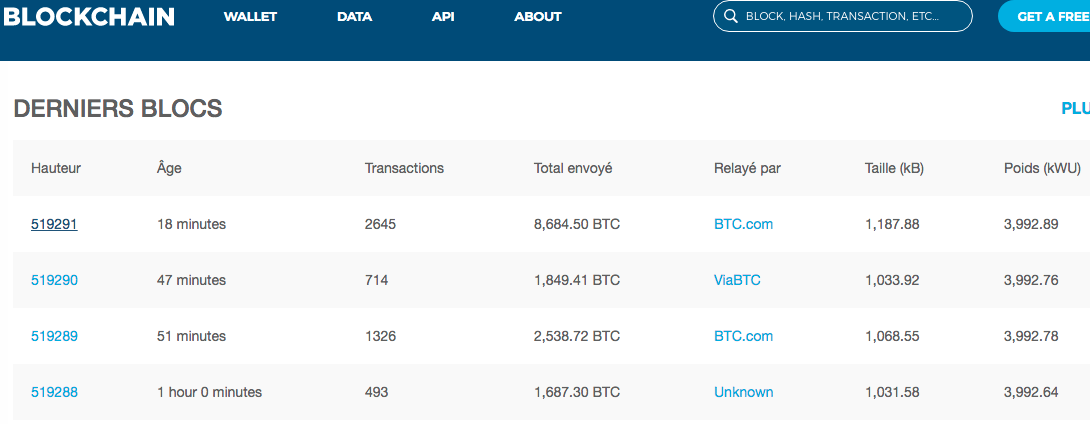
\includegraphics[width=12.5cm,height=5.25cm]{graphics/blockchain-info-2018-04-21-14-21-25.png}
\vskip 0.2cm
{\scriptsize\texttt{https://blockchain.info/fr}}
\end{center}

\end{columns}

\normalsize
\end{frame}

%%%%%%%%%%

\begin{frame}{\vskip -0.3cm\large La t\^ete d'un bloc du Bitcoin}

\begin{columns}
\column{\dimexpr\paperwidth-1pt}

\begin{center}
\vskip -0.3cm
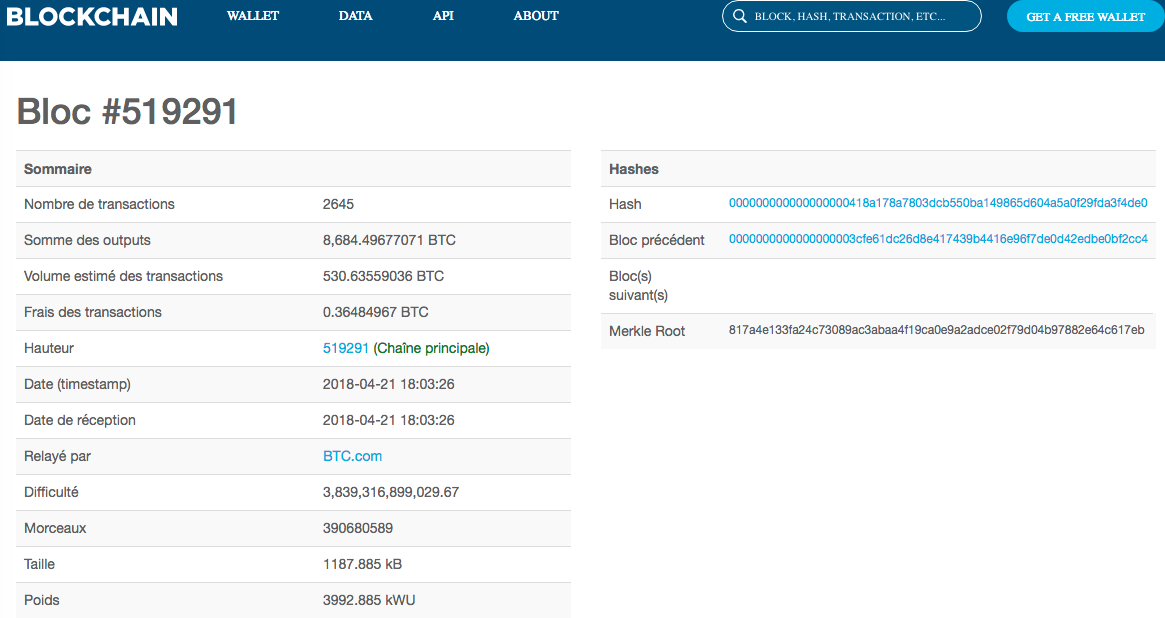
\includegraphics[width=12.5cm,height=7.0cm]{graphics/Bloc-bitcoin-519291-top.png}
\vskip -0.2cm
{\tiny\texttt{https://blockchain.info/fr}}
\end{center}

\end{columns}

\normalsize
\end{frame}

%%%%%%%%%%

\begin{frame}{}

\begin{columns}
\column{\dimexpr\paperwidth-1pt}

\begin{center}
\vskip 1.0cm
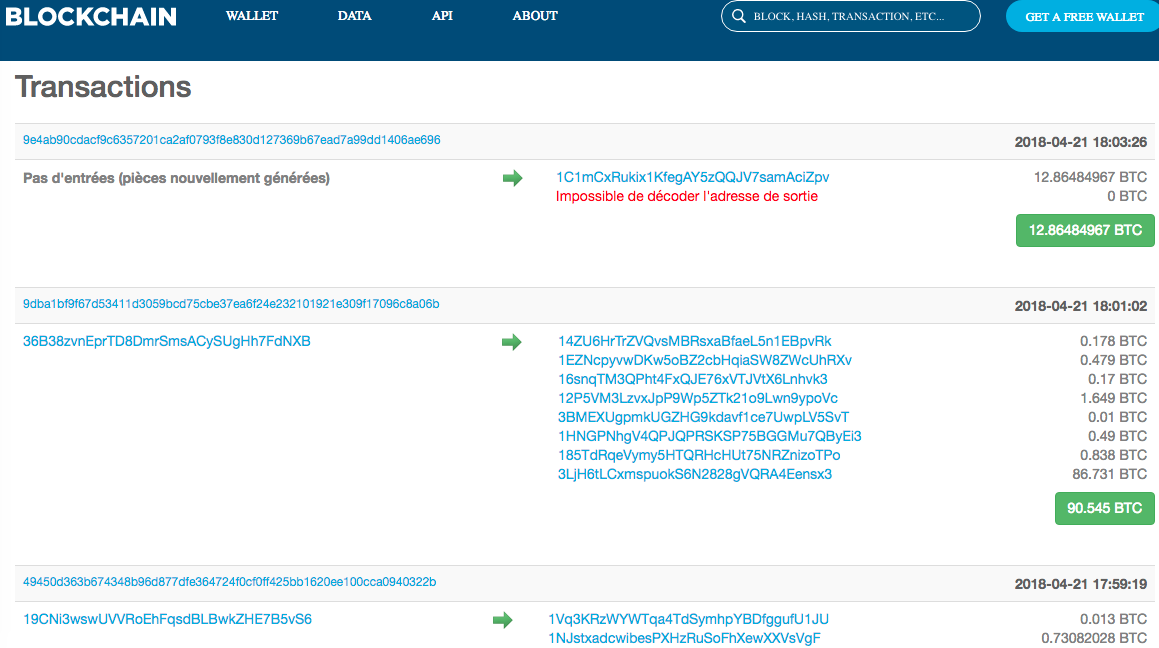
\includegraphics[width=12.5cm,height=7.0cm]{graphics/Bloc-bitcoin-519291-transactions-01.png}
\vskip 0.1cm
{\tiny\texttt{https://blockchain.info/fr}}
\end{center}

\end{columns}

\normalsize
\end{frame}

%%%%%%%%%%


%%%%%%%%%%

%\begin{frame}{\vskip -0.3cm\Large Organigramme du minage de bitcoins}
\begin{frame}{}

\begin{columns}
\column{\dimexpr\paperwidth-1pt}

\begin{center}
\vskip 0.7cm
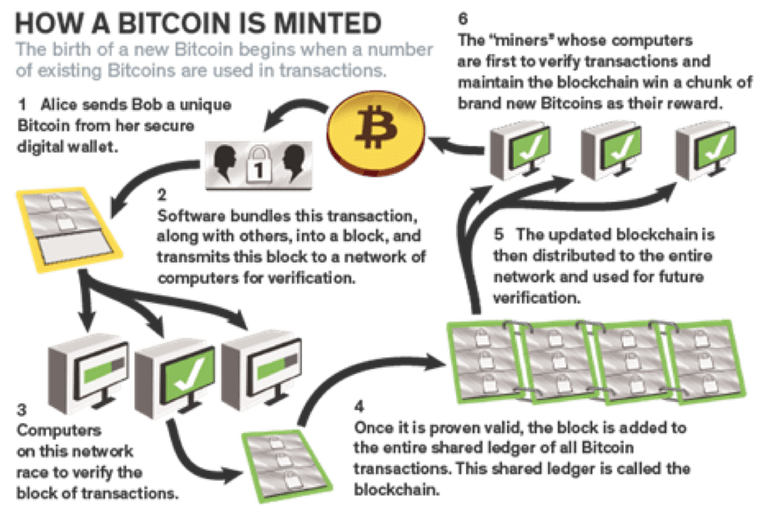
\includegraphics[width=12.5cm,height=8.0cm]{graphics/bitcoin-mining-process-graphic-overview.png}
\vskip -0.4cm
{\tiny\texttt{http://pointofsync.com/tag/bitcoin-mining/}}
\end{center}

\end{columns}

\normalsize
\end{frame}

%%%%%%%%%%


%%%%%%%%%%

\begin{frame}{\vskip -0.4cm\LARGE Comment faire du minage de bitcoins\vskip 0.05cm\normalsize(Comment un mineur cr\'ee un nouveau bloc)}

\scriptsize

\vskip 0.4cm
\textbf{\small Donn\'ees d'entr\'ees:}\;\;Des nouvelles transactions \;+\; Hash(\,bloc pr\'ec\'edent\,)

\vskip 0.5cm
\textbf{\small Travail:}
\begin{itemize}
\item
	{\footnotesize V\'erifier les nouvelles transactions contre l'histoire entri\`ere de la cha\^ine}
\item
	G\'en\'erer \`a plusieurs reprises un \guillemotleft\,nonce\,\guillemotright\,(nombre al\'eatoire) jusqu'\`a ce que
	\vskip -0.1cm
	{\scriptsize\begin{equation*}
	\textnormal{\footnotesize SHA-256}\left(
		\left\{\begin{array}{c}
			\textnormal{nouvelles transactions,}
			\\
			\textnormal{Hash(\,bloc pr\'ec\'edent\,),}
			\\
			\textnormal{{\color{red}nonce}}
		\end{array}\right\}
	\right)
	\quad < \;\;
	\begin{array}{c}
		\textnormal{{\color{red}difficult\'e} cibl\'ee}
		\\
		\textnormal{actuelle}
	\end{array}
	\end{equation*}}
\end{itemize}

\vskip 0.4cm
\textbf{\small Diffuser le {\color{red}nouveau bloc} au r\'eseau global du Bitcoin:}
\begin{itemize}
\item
	Les nouvelles transactions,\, Hash(\,bloc pr\'ec\'edent\,)
\item
	\mbox{}
	\vskip -0.5cm
	{\scriptsize\begin{equation*}
	\textnormal{\footnotesize Hash(\,nouveau bloc\,)}
	\;\; := \;\;
	\textnormal{\footnotesize SHA-256}\left(
		\left\{\begin{array}{c}
			\textnormal{nouvelles transactions,}
			\\
			\textnormal{Hash(\,bloc pr\'ec\'edent\,),}
			\\
			\textnormal{nonce}
		\end{array}\right\}
	\right)
	\end{equation*}}
\end{itemize}

\end{frame}
\normalsize

%%%%%%%%%%

\begin{frame}{\LARGE SHA-256 \normalsize(SHA \,=\, \guillemotleft\,Secure Hash Algorithm\,\guillemotright)}

\normalsize

\begin{itemize}
\item
	une fonction de hachage cryptographique
	\vskip -0.1cm
	{\scriptsize(comme une {\color{red}signature} de donn'ees, pour d\'etecter si une donn\'ee a \'et\'e modifi\'ee)}

\vskip 0.3cm
\item
	\`a une donn\'ee de taille arbitraire, associer une valeur de taille fixe (64 chiffres hexad\'ecimaux)

\vskip 0.3cm
\item
	``pratiquement'' injective (mais pas th\'eoriquement)

\vskip 0.3cm
\item
	donn\'ees diff\'erentes (m\^eme tr\`es similaires) \;$\leadsto$\; valeurs SHA-256 compl\`etement diff\'erentes

\vskip 0.3cm
\item
	exemples:
	\vskip 0.18cm{\tt\tiny
	{\footnotesize SHA256("Modernization is everywhere{\color{red}?}")}
	\vskip 0.02cm
	0x f531bba66e2bdf445dc15ece1e3507b4aada3bc71252c14580fd3562c8dc9293
	\vskip 0.3cm
	{\footnotesize SHA256("Modernization is everywhere{\color{red}!}")}
	\vskip -0.21cm
	0x 704bef9415ff0c2dd97acd439eefa9c7e123174cce8992e79480a4698c2771ab}
\end{itemize}

\end{frame}
\normalsize

%%%%%%%%%%

\begin{frame}{\Large SHA-256 \'etablit la continuit\'e de la cha\^ine de blocs enti\`ere du Bitcoin}

\begin{center}
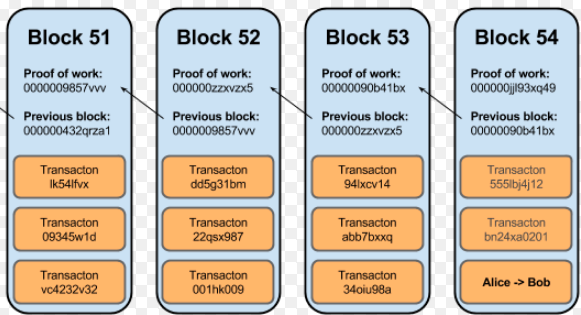
\includegraphics[width=10cm]{graphics/bitcoin-blockchain.png}
\vskip 0.1cm
{\tiny$^{\texttt{https://seekingalpha.com/article/4131577-iota-iot-capable-technology-alternative-blockchain}}$}
\end{center}

\end{frame}
\normalsize

%%%%%%%%%%


%%%%%%%%%%

\begin{frame}{\LARGE Le Bitcoin est s\'ecuris\'e.}

\normalsize

\begin{itemize}
\item
	SHA-256 garantit l'int\'egrit\'e des informations de
	toutes les transactions financi\`eres enregistr\'ees
	sur la cha\^ine de blocs enti\`ere du Bitcoin.

\vskip 0.4cm
\item
	On croire qu'il est impossible -- avec les technologies actuelles --
	de falsifier la base de donn\'ees {\color{red}distribu\'ee} du Bitcoin:
	\vskip 0.05cm
	\begin{itemize}
	\item
		Chaque mineur poss\`ede une copie enti\`ere de la cha\^ine de blocs du Bitcoin.
	\vskip 0.15cm
	\item
		Chaque nouveau bloc doit \^etre v\'erifi\'e par plus de la moiti\'e de mineurs
		avant d'\^etre ajout\'e officiellement sur la cha\^ine.
	\vskip 0.15cm
	\item
		Alors, pour falsifier des enregistrements Bitcoin, il faut pouvoir falsifier
		{\color{red}simultan\'ement plus de 50\%} des copies
		de la cha\^ine du Bitcoin distribu\'ees \`a travers du monde,
		ce qui est aujourd'hui consid\'er\'e comme impossible technologiquement.
	\end{itemize}
\end{itemize}

\end{frame}
\normalsize

%%%%%%%%%%



%%%%%%%%%%%%%%%%%%%%%%%%%%%%%%%%%%%%%%%%%%%%%%%%%%%

\begin{frame}{\vskip -0.1cm \huge Personne-ressource}

\large

\begin{center}
\begin{multicols}{2}
	\begin{minipage}{4.5cm}
	\vskip -2.6cm
	\begin{center}
	Pour plus d'information,
	\vskip -0.01cm
	\noindent
	veuillez contacter :
	\end{center}
	\end{minipage}
\columnbreak
	\begin{minipage}{4.0cm}
	\vskip -2.5cm
	\begin{center}
	For more information,
	\vskip -0.01cm
	\noindent
	please contact\!:
	\end{center}
	\end{minipage}
\end{multicols}
\end{center}

\begin{center}
\vskip 0.5cm
\textbf{\huge Kenneth\;\,Chu}
\vskip 0.15cm
%\texttt{\Large kenneth.chu@canada.ca}
\href{mailto:kenneth.chu@canada.ca}{\Large\color{darkBlue}\underline{\texttt{kenneth.chu@canada.ca}}}
\vskip 0.24cm
\texttt{\Large 613-852-7361}
\end{center}
%
\end{frame}
%\normalsize

%%%%%%%%%%%%%%%%%%%%%%%%%%%%%%%%%%%%%%%%%%%%%%%%%%%
%\begin{frame}{}
%
%\begin{center}
%\vskip 2.5cm
%\resizebox{\linewidth}{!}{\itshape Merci !!}
%\end{center}
%
%\begin{center}
%\vskip 0.5cm
%{\Large Kenneth Chu}
%\vskip 0.1cm
%\texttt{kenneth.chu@canada.ca}
%\vskip 0.1cm
%{\small Enqu\^{e}tes sp\'{e}ciales, transport, technologie et assurance de la qualit\'{e}, DMEE
%\vskip 0.0cm Special Surveys, Transportation, Technology and Quality Assurance, BSMD}
%\end{center}
%
%\end{frame}
%\normalsize
%
%%%%%%%%%%%%%%%%%%%%%%%%%%%%%%%%%%%%%%%%%%%%%%%%%%%


%%%%% ~~~~~~~~~~~~~~~~~~~~ %%%%%
\appendix

%%%%%%%%%%

\begin{frame}{}

\begin{columns}
\column{\dimexpr\paperwidth-1pt}

\begin{center}
\vskip 1.0cm
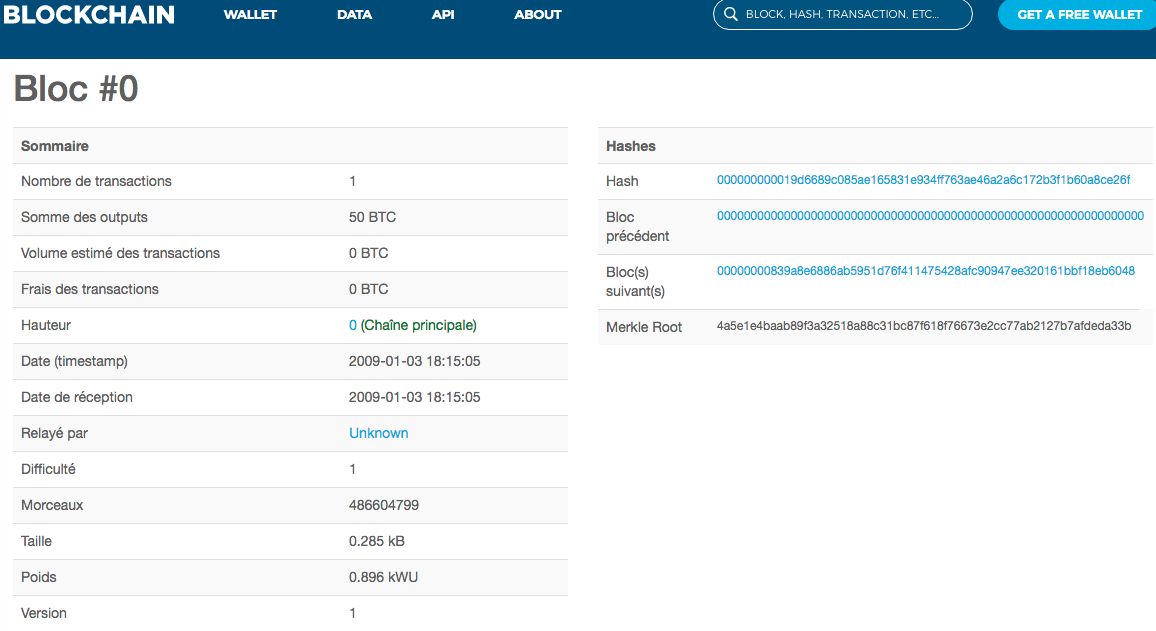
\includegraphics[width=12.5cm,height=7.0cm]{graphics/Bloc-bitcoin-0-top.png}
\vskip 0.1cm
{\tiny\texttt{https://blockchain.info/fr}}
\end{center}

\end{columns}

\normalsize
\end{frame}

%%%%%%%%%%

\begin{frame}{}

\begin{columns}
\column{\dimexpr\paperwidth-1pt}

\begin{center}
\vskip 1.0cm
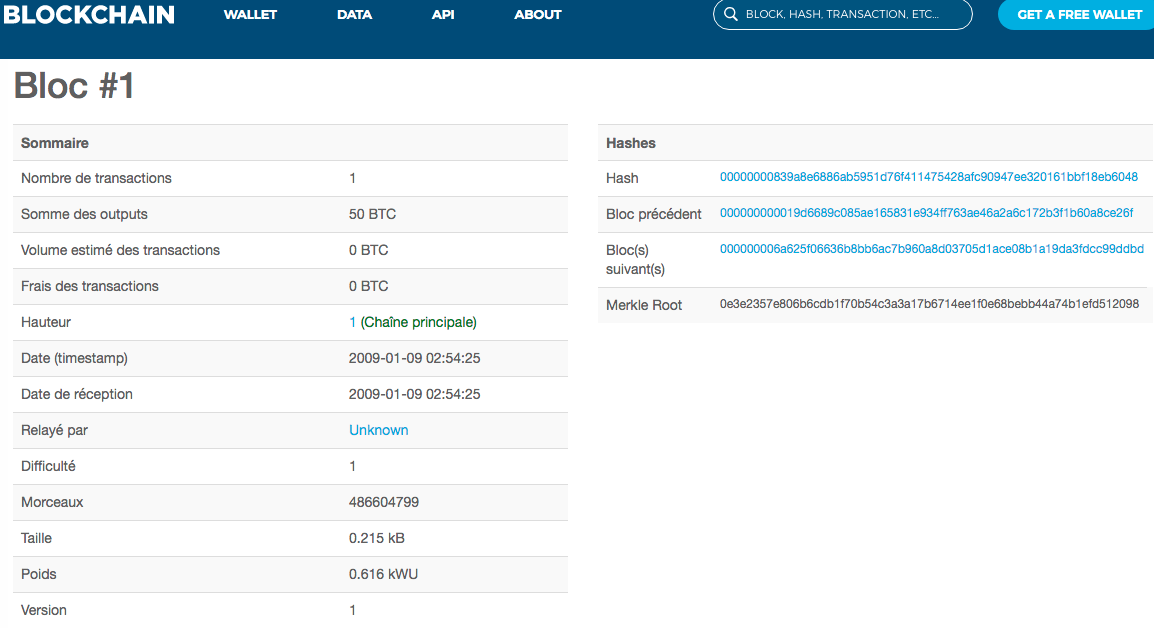
\includegraphics[width=12.5cm,height=7.0cm]{graphics/Bloc-bitcoin-1-top.png}
\vskip 0.1cm
{\tiny\texttt{https://blockchain.info/fr}}
\end{center}

\end{columns}

\normalsize
\end{frame}

%%%%%%%%%%

\begin{frame}{}

\begin{columns}
\column{\dimexpr\paperwidth-1pt}

\begin{center}
\vskip 1.0cm
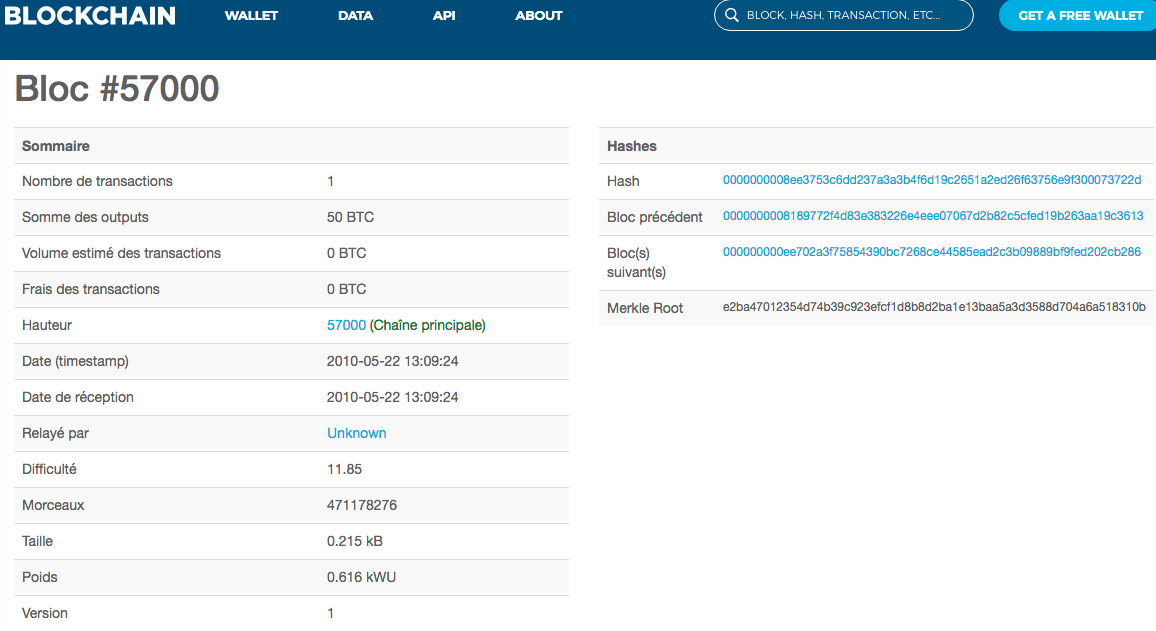
\includegraphics[width=12.5cm,height=7.0cm]{graphics/Bloc-bitcoin-57000-top.png}
\vskip 0.1cm
{\tiny\texttt{https://blockchain.info/fr}}
\end{center}

\end{columns}

\normalsize
\end{frame}

%%%%%%%%%%

\begin{frame}{}

\begin{columns}
\column{\dimexpr\paperwidth-1pt}

\begin{center}
\vskip 1.0cm
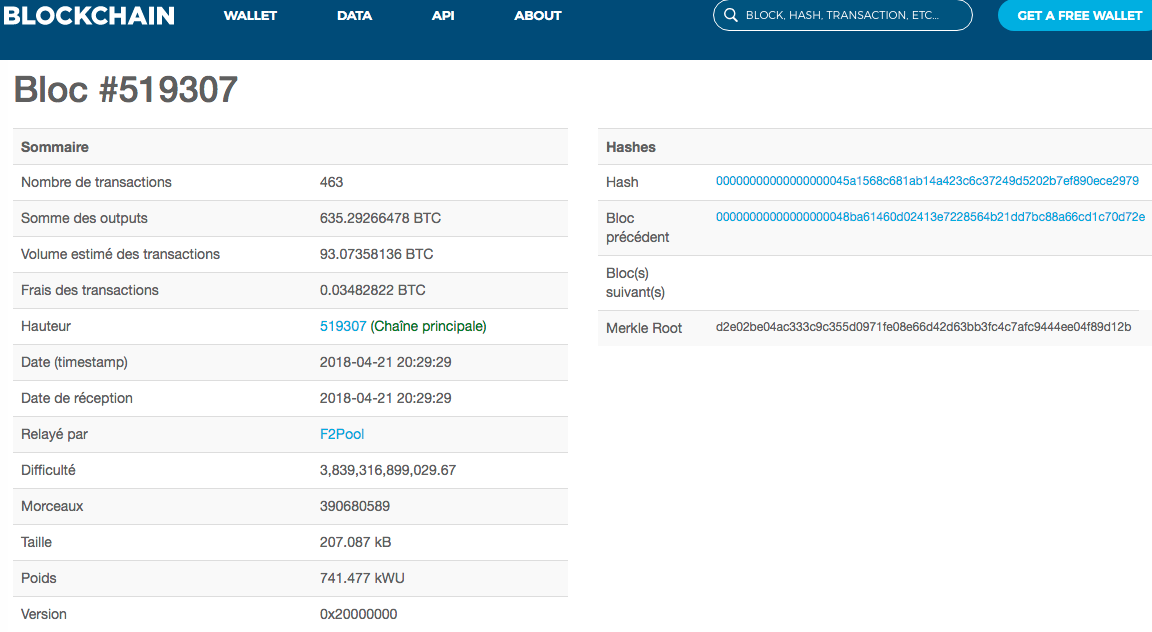
\includegraphics[width=12.5cm,height=7.0cm]{graphics/Bloc-bitcoin-519307-top.png}
\vskip 0.1cm
{\tiny\texttt{https://blockchain.info/fr}}
\end{center}

\end{columns}

\normalsize
\end{frame}

%%%%%%%%%%


%%%%%%%%%%%%%%%%%%%%%%%%%%%%%%%%%%%%%%%%%%%%%%%%%%

\end{document}

%%%%%%%%%%%%%%%%%%%%%%%%%%%%%%%%%%%%%%%%%%%%%%%%%%
